% !TeX root = ../tfg.tex
% !TeX encoding = utf8

\chapter{Teoría de procesamiento de señales} \label{chap:señales}
En oncología, la radiómica se ha consolidado como un enfoque prometedor al extraer características cuantitativas de imágenes médicas que pueden asociarse con resultados clínicos. Sin embargo, este análisis cuantitativo requiere una base matemática sólida que permita describir, transformar y procesar las señales contenidas en las imágenes.

En este capítulo se presentan los fundamentos de teoría de las señales necesarios para este propósito. Se abordan conceptos como la definición formal de señal, la transformada de Fourier, la operación y teorema fundamental de convolución y herramientas que permiten analizar y extraer información relevante de las imágenes médicas. Estos fundamentos son esenciales para construir descriptores radiómicos que se han utilizado en el Capítulo \ref{chap:aa-radiomica} de este trabajo y que han demostrado la mejor capacidad predictiva.

\section{Definición de señal}
El análisis de señales y sistemas es la base de muchos campos de la ingeniería, incluido el tratamiento de imágenes, ámbito de nuestro trabajo con imágenes médicas. 

\begin{definicion}
Una señal es una función que asigna valores reales y transmite información, pudiendo ser continua, $s : \mathbb{R}^n \rightarrow \mathbb{R}$, o discreta $s : \mathbb{Z}^n \rightarrow \mathbb{R}$.
\end{definicion}

En procesamiento de imágenes, una imagen digital se define como un sistema/señal discreta bidimensional. La imagen en sí puede extenderse más allá de imágenes bidimensionales hacia señales finitas $N$-dimensionales, como ocurre en las imágenes biomédicas 3D usadas en este trabajo. A menudo, una señal discreta toma valores en un subconjunto finito de puntos. Por ello, también se suelen considerar las señales discretas como aplicaciones $s: \{0, \dots, N_1-1\} \times \{0, \dots, N_d-1\}$, especialmente en el caso de imágenes y volúmenes tridimensionales.

Dado que una imagen es una señal discreta, muchas técnicas de procesamiento de señales también se utilizan en procesamiento de imágenes, incluyendo los \textit{Filtros Lineales}, que son herramientas principales en procesamiento de imágenes.

Un filtro se define como una transformación de una señal o imagen. En otras palabras, un filtro es un automorfismo sobreyectivo:

\begin{equation}
F : E \rightarrow E 
\end{equation}

donde $E$ es una señal.

Un filtro lineal es una aplicación lineal, es decir, un filtro es lineal si cumple la misma definición que cualquier aplicación lineal:

\begin{equation}
F(A + \lambda B) = F(A) + \lambda F(B) 
\end{equation}

donde $F$ es el filtro, $A$ y $B$ son dos señales y $\lambda$ es un escalar real. Un filtro es no lineal cuando esta relación se rompe.

\section{Operadores fundamentales}
\subsection{Transformada de Fourier}
La transformada de Fourier permite convertir una señal en una suma de distintas frecuencias. Utilizando la intensidad y la fase de esas frecuencias (o utilizando números complejos que permitan representar ambas) es posible con la transformada inversa volver a la señal original. Como una imagen digital es discreta, la DFT (transformada discreta de Fourier) es una aplicación que permite transformar una imagen en una matriz de intensidades de frecuencia y su fase que tiene las mismas dimensiones que la imagen original. El espectro de intensidad es una de las principales herramientas de análisis de imágenes, ya que permite ver qué frecuencias hay en la imagen. Esto la convierte en una herramienta útil para el análisis de texturas, al permitir visualizar las frecuencias de los patrones \parencite{azencott1997texture}. Además, el espectro de frecuencias suele ser mucho más disperso que la propia imagen, lo que lo convierte en una representación más eficiente.

A continuación se presentan las definiciones formales tanto de la transformada de Fourier en el dominio continuo como de su versión discreta multidimensional, empleada habitualmente en el procesamiento digital de imágenes:

\begin{definicion}[Transformada de Fourier continua]
Sea \( f \in L^1(\mathbb{R}) \) y $j$ la unidad imaginaria, la transformada de Fourier de \( f \) se define como:
\[
\hat{f}(\xi) = \int_{-\infty}^{\infty} f(x)\, e^{-2\pi j x \xi} \, dx, \quad \xi \in \mathbb{R}.
\]
La transformada inversa está dada por:
\[
f(x) = \int_{-\infty}^{\infty} \hat{f}(\xi)\, e^{2\pi j x \xi} \, d\xi, \quad x \in \mathbb{R}.
\]

En el caso m-dimensional, sea \( f \in L^1(\mathbb{R}^m) \), se define:
\[
F(\Omega_1, \Omega_2, \ldots, \Omega_m) = \int_{-\infty}^{\infty} \cdots \int_{-\infty}^{\infty} f(t_1, t_2, \ldots, t_m)\, e^{-j(\Omega_1 t_1 + \Omega_2 t_2 + \cdots + \Omega_m t_m)}\, dt_1 \cdots dt_m.
\]

donde $F$ representa la transformada multidimensional de Fourier, $m$ la dimensión multidimensional, $t_i$ las coordenadas originales en el espacio o tiempo y $\Omega_i$ las coordenadas en el dominio de frecuencias.

La transformada inversa está dada por:
\[
f(t_1, t_2, \ldots, t_m) = \frac{1}{(2\pi)^m} \int_{-\infty}^{\infty} \cdots \int_{-\infty}^{\infty} F(\Omega_1, \Omega_2, \ldots, \Omega_m)\, e^{j(\Omega_1 t_1 + \Omega_2 t_2 + \cdots + \Omega_m t_m)}\, d\Omega_1 \cdots d\Omega_m.
\]
\end{definicion}

\begin{definicion}[Transformada Discreta de Fourier multidimensional]

Sea \( f : \{0, 1, \ldots, N_1 - 1\} \times \cdots \times \{0, 1, \ldots, N_m - 1\} \to \mathbb{C} \) una señal discreta m-dimensional. La Transformada Discreta de Fourier m-dimensional normalizada está dada por:
\[
F(K_1, K_2, \ldots, K_m) = \frac{1}{\sqrt{N_1 \cdot \ldots \cdot N_m}} \sum_{n_1=0}^{N_1-1} \cdots \sum_{n_m=0}^{N_m-1} f(n_1, n_2, \ldots, n_m) \, e^{-j \frac{2\pi}{N_1} n_1 K_1 - j\frac{2\pi}{N_2} n_2 K_2 - \cdots - j \frac{2\pi}{N_m} n_m K_m},
\]
para \( 0 \leq K_i \leq N_i -1, \; i=1,2,\ldots,m. \)

La \textbf{transformada inversa} está dada por:
\[
f(n_1, n_2, \ldots, n_m) = \frac{1}{\sqrt{N_1 \cdot \ldots \cdot N_m}} \sum_{K_1=0}^{N_1-1} \cdots \sum_{K_m=0}^{N_m-1} F(K_1, K_2, \ldots, K_m) \, e^{j \frac{2\pi}{N_1} n_1 K_1 + j \frac{2\pi}{N_2} n_2 K_2 + \cdots + j \frac{2\pi}{N_m} n_m K_m},
\]
para \( 0 \leq n_i \leq N_i -1, \; i=1,2,\ldots,m. \)


donde \( m \) es el número de dimensiones, \( n_i \) son los índices espaciales o temporales en la dimensión \( i \) y \( K_i \) son los índices de frecuencia discreta en la dimensión \( i \).
\end{definicion}



\subsection{La operación de convolución} \label{subsec:op-convolucion} 

En su forma más general, la convolución es una operación que tiene como argumento dos funciones de variable real \parencite{Goodfellow-et-al-2016}. Sean $f, g : \mathbb{R} \rightarrow \mathbb{R}$ dos funciones de variable real, la convolución continua de ambas funciones se denota por $(f * g)$ a su convolución y se define como:

\begin{equation}
s(t) = (f * g) = \int_{-\infty}^{\infty} f(a) \, g(t - a) \, da
\end{equation}

El primer argumento, es decir $f$, se le conoce como la entrada, y el segundo, $g$, es el núcleo o \textit{kernel} o \textit{filtro} de la convolución. Al resultado se suele llamar mapa de características o \textit{feature map}.

En implementaciones prácticas, se trabaja con datos discretos ya que con un ordenador no podemos trabajar con datos continuos. Por tanto, definimos naturalmente tras la definición anterior de convolución continua, la convolución discreta:

\begin{equation}
s(t) = (f * g) = \sum_{s=-\infty}^{\infty} f(a) \, g(t - a).
\end{equation}

En aplicaciones de aprendizaje automático, la entrada suele ser un array multidimensional de datos y el kernel es un array multidimensional de parámetros que se aprenden. Cada elemento de la entrada y del kernel debe especificarse de forma explícita, pero se suele suponer que estas funciones son cero fuera del rango finito de valores que se almacenan. Esto permite en la práctica implementar la suma infinita como una suma sobre un número finito de elementos.

En muchos casos se aplican convoluciones sobre más de un eje a la vez. Por ejemplo, con una imagen $I$ como entrada y un kernel $K$ bidimensionales se define:

\begin{equation}
S(i,j) = (I * K)(i,j) = \sum_m \sum_n I(m,n) \, K(i - m, j - n).
\end{equation}

La propiedad conmutativa de la convolución permite escribir de forma equivalente:

\begin{equation}
S(i,j) = (K * I)(i,j) = \sum_m \sum_n  K(m,n) \,I(i - m, j - n).
\end{equation}

Normalmente, esta segunda forma resulta más sencilla de implementar, ya que reduce la variación en los índices válidos de $m$ y $n$.

Aunque la convolución es conmutativa en sentido matemático, en implementaciones prácticas suele usarse una operación relacionada llamada \emph{correlación cruzada}. Esta se define de forma similar a la convolución pero omite el volteo del kernel:

\begin{equation}
S(i,j) = (I * K)(i,j) = \sum_m \sum_n I(i + m, j + n) \, K(m,n).
\end{equation}

En aprendizaje automático, el algoritmo de entrenamiento ajusta los valores del kernel en la ubicación correcta. Un algoritmo basado en convolución con volteo del kernel aprenderá un kernel volteado respecto a uno aprendido por un algoritmo que no aplique el volteo. Además, es raro usar la convolución como única operación en redes neuronales; suele combinarse con otras funciones, y la composición de estas no conmutará en general, independientemente de si la convolución voltea el kernel o no.

La convolución discreta puede verse como una forma de multiplicación por una matriz. Sin embargo, esta matriz tiene una estructura especial: muchas de sus entradas están restringidas a ser iguales a otras. 

Antes de continuar vamos a dar dos definiciones \parencite{gray2006toeplitz}: 

\begin{definicion}
Una \textbf{matriz de Toeplitz} es una matriz $n \times n$,  $T_n = [t_{k,j}; \, k, j = 0, 1, \ldots, n-1]$  
donde $t_{k,j} = t_{k - j}$, es decir, una matriz de la siguiente forma:


\begin{equation}
T_n = 
\begin{bmatrix}
t_0 & t_{-1} & t_{-2} & \cdots & t_{-(n-1)} \\
t_1 & t_0 & t_{-1} & \cdots & \vdots \\
t_2 & t_1 & t_0 & \cdots & \vdots \\
\vdots & \vdots & \vdots & \ddots & \vdots \\
t_{n-1} & \cdots & \cdots & \cdots & t_0
\end{bmatrix}.
\end{equation}
\end{definicion}

Un caso especial común de las matrices de Toeplitz, que resulta en una simplificación significativa y juega un papel fundamental en el desarrollo de resultados más generales, ocurre cuando cada fila de la matriz es un desplazamiento cíclico hacia la derecha de la fila anterior, de forma que $t_k = t_{-(n-k)} = t_{k-n}$ para $k = 1, 2, \ldots, n-1$. Las definimos como:
\begin{definicion}
Una \textbf{matriz de circulante} es una matriz $n \times n$,  $C_n = [t_{k,j}; \, k, j = 0, 1, \ldots, n-1]$  donde $t_k = t_{-(n-k)} = t_{k-n}$ para $k = 1, 2, \ldots, n-1$, es decir, una matriz de la siguiente forma:

\begin{equation}
C_n = 
\begin{bmatrix}
t_0 & t_{-1} & t_{-2} & \cdots & t_{-(n-1)} \\
t_{-(n-1)} & t_0 & t_{-1} & \cdots & \vdots \\
t_{-(n-2)} & t_{-(n-1)} & t_0 & \cdots & \vdots \\
\vdots & \vdots & \vdots & \ddots & \vdots \\
t_{-1} & t_{-2} & \cdots & \cdots & t_0
\end{bmatrix}.
\end{equation}
\end{definicion}

Las matrices circulantes surgen, por ejemplo, en aplicaciones que involucran la transformada discreta de Fourier (DFT) y en el estudio de códigos cíclicos para corrección de errores.




Continuando con el argumento anterior, en una dimensión, la convolución discreta corresponde a matrices de Toeplitz, mientras que en dos dimensiones se relaciona con matrices circulantes por bloques. Estas restricciones generan matrices muy dispersas, donde la mayoría de las entradas son cero, reflejando el hecho de que el kernel suele ser mucho más pequeño que la entrada.  

Cualquier algoritmo de red neuronal que funcione con multiplicación de matrices funcionará también con convolución sin requerir cambios adicionales. Las redes convolucionales típicas, no obstante, implementan optimizaciones específicas para procesar entradas de gran tamaño de forma eficiente, aunque estas optimizaciones no son estrictamente necesarias desde el punto de vista teórico.


\subsection{Teorema fundamental de la convolución}
La transformada de Fourier tiene propiedades útiles, como por ejemplo que los operadores lineales tienen equivalentes lineales en el dominio recíproco. El filtrado lineal consiste en realizar operaciones en el dominio de la frecuencia, como por ejemplo atenuar o realzar ciertas frecuencias.

El teorema de la convolución establece que cualquier multiplicación puntual en un dominio equivale a una convolución en el otro dominio.

\begin{equation}
\mathcal{F}\{f * g\} = \mathcal{F}\{f\} \cdot \mathcal{F}\{g\} \tag{1.11}
\end{equation}

\begin{equation}
\mathcal{F}\{f \cdot g\} = \mathcal{F}\{f\} * \mathcal{F}\{g\} \tag{1.12}
\end{equation}


Una aplicación de este teorema es que cualquier convolución puede implementarse de manera eficiente realizando una multiplicación en el dominio espectral tras una transformada rápida de Fourier (FFT). La aplicación generalizada de la DFT a la convolución y al análisis espectral se debe a la existencia de algoritmos rápidos para su implementación. Estos métodos se denominan FFT \parencite{krishna2017digital}. Esto implica que cualquier filtro basado en frecuencia puede modelarse mediante una convolución con una matriz que representa la respuesta al impulso del filtro.

\subsection{Definición formal del producto de convolución}

Vamos a definir formalmente el producto de convolución. Introducimos previamente la siguiente notación. En adelante, dado $p \in [1,\infty]$, notaremos $p^* \in [1,\infty]$ como aquel número que verifique $1/p + 1/p^* = 1$, si $1 < p < \infty$, $p^* = \infty$ si $p = 1$ y $p^* = 1$ si $p = \infty$.
\vspace{0.3cm}

\begin{definicion}
Sean $f, g \in L(\mathbb{R}^N)$, y sea $H \in L(\mathbb{R}^{2N})$ dada por $H(x,y) = f(x - y)g(y)$, p.c.t. $(x,y) \in \mathbb{R}^{2N}$.  

Dado $x \in \mathbb{R}^N$ diremos que la \textit{convolución} de $f$ y $g$ está definida en $x$, y escribimos $\exists(f * g)$, cuando $H_x \in L_1(\mathbb{R}^N)$, en cuyo caso, se define su convolución por
\[
(f * g)(x) = \int_{\mathbb{R}^N} f(x - y)g(y) \, dy
\]

\end{definicion}

En tal caso, es fácil comprobar (mediante la invarianza de la integral por isometrías) que $\exists(g * f)(x)$ y $(f * g)(x) = (g * f)(x)$.

\vspace{0.3cm}

Diremos que existe la convolución de $f$ y $g$ y escribimos $\exists(f * g)$, cuando $\exists(f * g)(x)$ p.c.t. $x \in \mathbb{R}^N$, en cuyo caso, $f * g \in L(\mathbb{R}^N)$ y viene dada por
\[
(f * g)(x) = \int_{\mathbb{R}^N} f(x - y)g(y) \, dy \quad \text{p.c.t. } x \in \mathbb{R}^N
\]

\vspace{0.5cm}

Antes de ver algunos resultados sobre la existencia del producto de convolución de dos funciones, enunciemos este lema:

\begin{lema}[Continuidad de las traslaciones] 
Sea $1 \leq p < \infty$ y $f \in L_p(\mathbb{R}^N)$. Para $y \in \mathbb{R}^N$ definimos $f_{[y]} \in L_p(\mathbb{R}^N)$ por $f_{[y]}(x) = f(x - y)$ p.c.t. $x \in \mathbb{R}^N$. \label{lema:lema} 
\end{lema}


\vspace{0.3cm}

\begin{proposicion}[Existencia en todo punto]
Si $f \in L_p(\mathbb{R}^N)$ y $g \in L_{p^*}(\mathbb{R}^N)$, entonces

\begin{itemize}
    \item[(a)] $\exists(f * g)(x)$ para todo $x \in \mathbb{R}^N$.
    \item[(b)] $\|(f * g)\|_\infty \leq \|f\|_p \|g\|_{p^*}$ para todo $x \in \mathbb{R}^N$.
    \item[(c)] $f * g : \mathbb{R}^N \to \mathbb{C}$ es uniformemente continua.
\end{itemize}
\end{proposicion}

\textit{Demostración:}
\vspace{0.2cm}
a) Si $1 < p < \infty$, se tiene, por la desigualdad de Hölder,
\[
\int |f(x - y)||g(y)| \, dy \leq \left( \int |f(x - y)|^p \, dy \right)^{1/p} \left( \int |g(y)|^{p^*} \, dy \right)^{1/p^*} < \infty,
\]
y la desigualdad se verifica para todo $x \in \mathbb{R}^N$.

\vspace{0.2cm}

Para $p = 1$, acotamos con la norma infinito
\[
\int |f(x - y)||g(y)| \, dy \leq \|g\|_\infty \int |f(x - y)| \, dy < \infty.
\]

Para $p = \infty$ es análogo al caso anterior.

\vspace{0.4cm}

b) $|(f * g)(x)| \leq \int |f(x - y)g(y)| \, dy$, y por el apartado anterior se tiene la desigualdad buscada.

\vspace{0.4cm}

c) Se verifica, aplicando de nuevo la desigualdad de Hölder,
\[
|(f * g)(u) - (f * g)(v)| = \left| \int (f(u - y) - f(v - y)) g(y) \, dy \right|
\]
\[
\leq \int |f(u - y) - f(v - y)| |g(y)| \, dy
\]
\[
\leq \left( \int |f(u - y) - f(v - y)|^p \, dy \right)^{1/p} \|g\|_{p^*} = \|f_u - f_v\|_p \|g\|_{p^*}.
\]

\vspace{0.3cm}

Si $\|g\|_{p^*} = 0$, la continuidad uniforme es clara. En caso contrario, dado $\varepsilon > 0$, por el Lema \ref{lema:lema} existe un $\delta > 0$ tal que si $\|u - v\| < \delta$, entonces $\|f_u - f_v\|_p < \varepsilon / \|g\|_{p^*}$. Aplicado a lo que acabamos de calcular, obtenemos
\[
|(f * g)(u) - (f * g)(v)| < \frac{\varepsilon}{\|g\|_{p^*}} \|g\|_{p^*} = \varepsilon. \tag*{$\Box$}
\]

\begin{proposicion}[Existencia c.p.d.]
Sea $f \in L_p(\mathbb{R}^N)$ con $1 \leq p \leq \infty$ y $g \in L_1(\mathbb{R}^N)$. Entonces existe $f * g$, que pertenece a $L_p(\mathbb{R}^N)$, y $\|f * g\|_p \leq \|f\|_p \|g\|_1$.
\end{proposicion}

\vspace{0.3cm}

\textit{Demostración.} En primer lugar, si $p = \infty$, entonces $p^* = 1$ y la tesis se obtiene a partir de la existencia en todo punto.

\vspace{0.3cm}

Supongamos que $p = 1$. Aplicando el Teorema de Fubini para funciones medibles positivas obtenemos que
\begin{equation}
\int_{\mathbb{R}^{2N}} |f(x - y)g(y)| \, d(x,y) = \int_{\mathbb{R}^N} |g(y)| \left( \int_{\mathbb{R}^N} |f(x - y)| \, dx \right) dy = \|f\|_1 \|g\|_1 < \infty. \label{eq:igualdad}
\end{equation}

Por tanto, por el Teorema de Fubini para funciones integrables, obtenemos que $(f * g)(x)$ existe para casi todo $x \in \mathbb{R}^N$. Además, la igualdad \eqref{eq:igualdad} concluye que
\[
\|f * g\|_1 = \int_{\mathbb{R}^N} \left| \int_{\mathbb{R}^N} f(x - y)g(y) \, dy \right| dx \leq \int_{\mathbb{R}^N} \int_{\mathbb{R}^N} |f(x - y)g(y)| \, dy \, dx = \|f\|_1 \|g\|_1.
\]

\vspace{0.3cm}

Por último, supongamos que $p > 1$. Como consecuencia de la desigualdad de Hölder, tenemos que
\[
\int_{\mathbb{R}^N} |f(x - y)g(y)| \, dy \leq \left( \int_{\mathbb{R}^N} |f(x - y)|^p \, dy \right)^{1/p} \left( \int_{\mathbb{R}^N} |g(y)|^{p^*} \, dy \right)^{1/p^*}
\]
\[
= \|f\|_p \|g\|_{p^*}.
\]

para casi todo $x \in \mathbb{R}^N$, donde se ha utilizado el caso anterior sobre $|f|^p$. Por tanto, existe $(f * g)(x)$ p.c.t. $x \in \mathbb{R}^N$. Además, esta cota junto con el caso previo proporcionan la desigualdad
\[
\|f * g\|_p^p \leq \int_{\mathbb{R}^N} \left( \int_{\mathbb{R}^N} |f(x - y)g(y)| \, dy \right)^p dx
\]
\[
\leq \|g\|_{p^*}^p \int_{\mathbb{R}^N} (|f|^p * |g|)(x) \, dx
\]
\[
\leq \|g\|_{p^*}^p \|g\|_1 \|f\|_p^p = \|f\|_p^p \|g\|_1^p. \tag*{$\Box$}
\]

\vspace{0.4cm}

El producto de convolución dota a $L_1(\mathbb{R}^N)$ de una operación con múltiples propiedades que se recogen en el siguiente resultado.

\vspace{0.3cm}

\begin{proposicion}
La aplicación $(f,g) \mapsto f * g$ de $L_1(\mathbb{R}^N) \times L_1(\mathbb{R}^N)$ en $L_1(\mathbb{R}^N)$ es una aplicación bilineal, conmutativa y asociativa que no tiene elemento neutro. Además, para cada $f, g \in L_1(\mathbb{R}^N)$ se verifica la desigualdad $\|f * g\|_1 \leq \|f\|_1 \|g\|_1$. En particular, esta aplicación es continua.

\end{proposicion}


\section{Interpretación de la teoría de Fourier y convolución en imágenes}

La teoría de Fourier puede ser muy compleja en su formulación matemática, pero tiene ideas conceptuales sorprendentemente simples y visuales que facilitan su comprensión. En esta sección se presenta una visión intuitiva, especialmente aplicada a imágenes espaciales, que complementa la formulación formal que vimos antes.

La idea esencial de la transformada de Fourier es que \emph{cualquier señal}, incluida una imagen, puede expresarse como la suma de una serie de ondas sinusoidales \parencite{leharFourier}. En imágenes, estas son variaciones sinusoidales de brillo a lo largo del espacio.

Cada componente sinusoidal se caracteriza por tres parámetros:
\begin{itemize}
    \item \textbf{Frecuencia espacial}: Este parámetro describe la frecuencia con la que el brillo modula a través del espacio (por ejemplo, a lo largo del eje x). Una mayor frecuencia espacial significa que el patrón sinusoidal tiene más ciclos en la misma distancia, como se ve al comparar dos senoides con diferentes frecuencias espaciales.
    \item \textbf{Magnitud}: La magnitud de la sinusoide corresponde a su contraste, que es la diferencia entre los picos más oscuros y más brillantes de la imagen. Una magnitud negativa indica una inversión de contraste, donde los brillos se vuelven oscuros y viceversa.
    \item \textbf{Fase}: La fase representa cuánto se desplaza la onda con respecto al origen, es decir, cuánto se desplaza la sinusoide hacia la izquierda o hacia la derecha
\end{itemize}

\begin{figure}[!htbp]
    \centering
    \begin{subfigure}[b]{0.45\textwidth}
        \centering
        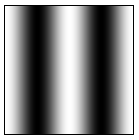
\includegraphics[width=\textwidth]{img/sin_baja_frec.png}
        \caption{Ejemplo de patrón sinusoidal de baja frecuencia espacial.}
        \label{fig:sinusoide_baja}
    \end{subfigure}
    \hfill
    \begin{subfigure}[b]{0.45\textwidth}
        \centering
        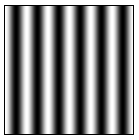
\includegraphics[width=\textwidth]{img/sin_alta_frec.png}
        \caption{Ejemplo de patrón sinusoidal de más alta frecuencia espacial.}
        \label{fig:sinusoide_alta}
    \end{subfigure}
    \caption{Comparación entre patrones sinusoidales de distinta frecuencia espacial \parencite{leharFourier}.}
    \label{fig:comparacion_sinusoidales}
\end{figure}

El concepto clave es que incluso formas complejas pueden reconstruirse sumando senos y cosenos de diferentes frecuencias, amplitudes y fases.

Las frecuencias espaciales más altas corresponden a variaciones más rápidas en el brillo (detalles finos), mientras que las bajas representan transiciones suaves o graduales. El límite máximo de frecuencia que puede codificar una imagen digital está determinado por su resolución (el tamaño del píxel), conocido como la \emph{frecuencia de Nyquist}.

La transformada de Fourier no codifica solo una onda, sino todas las frecuencias presentes en la imagen. El resultado es un \emph{espectro de frecuencias}, donde:
\begin{itemize}
    \item La posición indica la frecuencia espacial.
    \item La altura (o brillo) del pico indica la amplitud o contraste.
\end{itemize}

Por tanto, una señal que contiene una única frecuencia espacial de frecuencia $f$ se representa como un único pico en el punto $f$ a lo largo del eje de frecuencias espaciales

El \emph{término DC} correspondiente a la frecuencia cero, que representa el brillo medio en toda la imagen. Un término de DC cero significaría una imagen con un brillo medio de cero, lo que significaría que la sinusoide alterna entre valores positivos y negativos en la imagen de brillo. Pero como no existe el brillo negativo, todas las imágenes reales tienen un término de DC positivo.

En imágenes 2D, la transformada se realiza aplicando transformadas 1D a filas y luego a columnas. El resultado es una imagen en el \emph{dominio de la frecuencia}, donde cada punto representa una frecuencia espacial (con magnitud y orientación).
\begin{figure}[!htbp]
    \centering
    \begin{subfigure}[b]{0.45\textwidth}
        \centering
        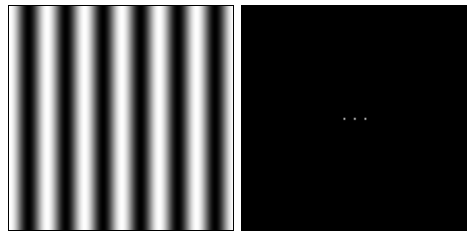
\includegraphics[width=\textwidth]{img/f1.png}
        \caption{Patrón sinusoidal vertical y su transformada de Fourier.}
        \label{fig:sinusoide_vertical}
    \end{subfigure}
    \hfill
    \begin{subfigure}[b]{0.45\textwidth}
        \centering
        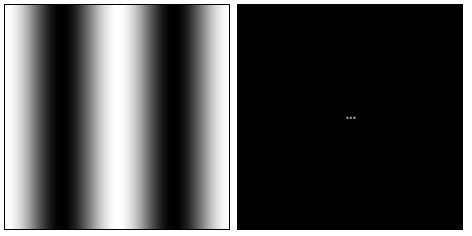
\includegraphics[width=\textwidth]{img/f2.png}
        \caption{Patrón sinusoidal con frecuencia espacial más baja y su transformada.}
        \label{fig:sinusoide_baja_frecuencia}
    \end{subfigure}

    \vspace{0.5cm}

    \begin{subfigure}[b]{0.45\textwidth}
        \centering
        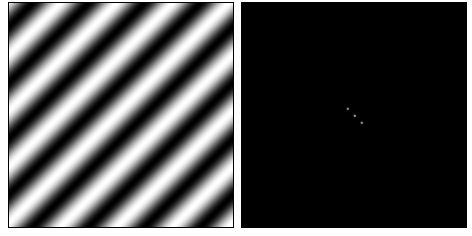
\includegraphics[width=\textwidth]{img/f3.png}
        \caption{Patrón sinusoidal inclinado y su transformada de Fourier.}
        \label{fig:sinusoide_inclinada}
    \end{subfigure}
    \hfill
    \begin{subfigure}[b]{0.45\textwidth}
        \centering
        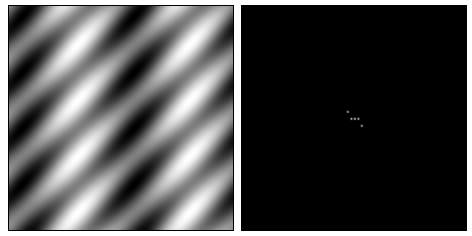
\includegraphics[width=\textwidth]{img/f4.png}
        \caption{Combinación de dos patrones sinusoidales y su transformada.}
        \label{fig:suma_sinusoidales}
    \end{subfigure}

    \caption{Comparación de distintos patrones sinusoidales y sus transformadas de Fourier \parencite{leharFourier}.}
    \label{fig:cuadricula_sinusoidales}
\end{figure}


En la imagen \ref{fig:sinusoide_vertical} se observan franjas verticales de luminancia alternante ya que es una onda sinusoidal en dirección horizontal. En su transformada de Fourier, observamos dos picos simétricos alrededor del centro (el término DC), alineados horizontalmente. Esto indica la frecuencia espacial dominante y su dirección. La separación de los picos con respecto al centro representa la frecuencia espacial: a mayor distancia, mayor frecuencia. 



En la imagen \ref{fig:sinusoide_baja_frecuencia} se observa que las franjas son más anchas porque la frecuencia espacial es menor. En la transformada de Fourier, los dos picos laterales están más cerca del centro. Esto muestra cómo la separación de los picos en el dominio de Fourier está inversamente relacionada con la frecuencia espacial en la imagen original.



En la imagen \ref{fig:sinusoide_inclinada} el patrón de brillo muestra franjas inclinadas. En su transformada de Fourier, los dos picos aparecen simétricamente alineados en la dirección perpendicular a las franjas. La orientación de las estructuras en la imagen espacial se codifica en la dirección de los picos en el dominio de la frecuencia.



En la imagen \ref{fig:suma_sinusoidales} se ve un patrón más complejo, resultado de sumar dos ondas sinusoidales con distintas direcciones y frecuencias. La transformada de Fourier muestra picos en las posiciones correspondientes a cada componente. Esto ilustra cómo la transformada de Fourier combina aditivamente las frecuencias presentes en la imagen.

\subsubsection{Filtro de Fourier}

Vamos a mostrar cómo se puede utilizar la transformada de Fourier para realizar operaciones de filtrado con el fin de ajustar el contenido de frecuencia espacial de una imagen. Comenzamos con una imagen de entrada mostrada en \ref{fig:tranf_inversa_3}, y realizamos una transformada de Fourier sobre ella, luego hacemos una transformada inversa para reconstruir la imagen original. Esta imagen reconstruida es idéntica, píxel a píxel, a la imagen de brillo original.

\begin{figure}[!htbp]
    \centering
    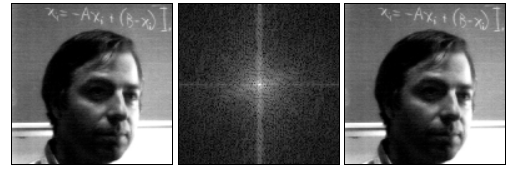
\includegraphics[width=0.6\textwidth]{img/f5.png}
    \caption{Transformada de Fourier directa e inversa de la imagen de entrada. }
    \label{fig:tranf_inversa_3}
\end{figure}



A continuación mostraremos cómo podemos manipular la imagen transformada para ajustar su contenido en frecuencia espacial y luego realizar la transformada inversa para producir la imagen filtrada. Comenzamos con un filtro paso-bajo, es decir, un filtro que permite pasar las componentes de baja frecuencia espacial pero elimina las de alta frecuencia. Dado que las componentes de baja frecuencia se concentran cerca del punto DC central, basta con definir un radio alrededor de dicho punto y anular el resto de la imagen de Fourier. Aplicando la transformada inversa obtenemos la imagen filtrada paso-bajo \ref{fig:pasabajas}.

\begin{figure}[!htbp]
    \centering
    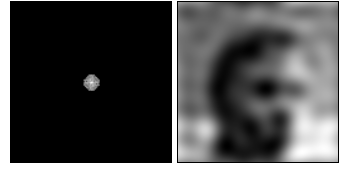
\includegraphics[width=0.6\textwidth]{img/f6.png}
    \caption{Filtrado paso-bajo en el dominio de Fourier y su resultado tras la transformada inversa. }
    \label{fig:pasabajas}
\end{figure}

Podemos ver que la imagen filtrada con paso-bajo aparece difuminada, preservando las zonas amplias y suaves de baja frecuencia pero perdiendo los bordes definidos y detalles nítidos. 



A continuación probamos el caso opuesto en la imagen \ref{fig:pasaaltas}: un filtro paso-alto, usando el mismo umbral de frecuencia espacial para definir el radio en la imagen de Fourier. Eliminamos todas las componentes de frecuencia espacial más bajas, preservando únicamente las componentes de frecuencia espacial más alta. Después de la transformada inversa obtenemos el efecto del filtrado paso-alto, que conserva los bordes nítidos de la imagen original pero pierde las grandes regiones uniformes de brillo.

\begin{figure}[!htbp]
    \centering
    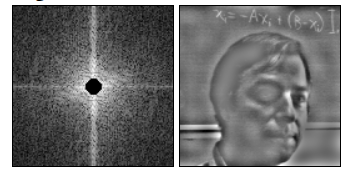
\includegraphics[width=0.6\textwidth]{img/f7.png}
    \caption{Filtrado paso-alto en el dominio de Fourier y su resultado tras la transformada inversa.}
    \label{fig:pasaaltas}
\end{figure}

Si sumamos la imagen con filtro paso-bajo y la filtrada con paso-alto (ambas ya transformadas inversas), obtenemos exactamente la imagen original no filtrada. Son imágenes complementarias: cada una codifica la parte de la información que le falta a la otra.


A continuación mostraremos en \ref{fig:pasabanda1} un filtrado paso-banda, que preserva únicamente las frecuencias espaciales que caen dentro de una banda: mayores que un corte bajo pero menores que un corte alto.

\begin{figure}[!htbp]
    \centering
    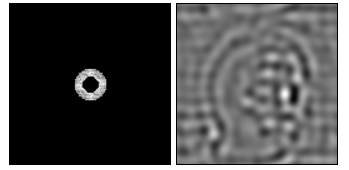
\includegraphics[width=0.6\textwidth]{img/f8.png}
    \caption{Primer ejemplo de filtrado paso-banda en el dominio de Fourier y su resultado tras la transformada inversa.}
    \label{fig:pasabanda1}
\end{figure}

La simulación \ref{fig:pasabanda2} es igual a la anterior pero usando una banda de frecuencias espaciales más estrecha.

\begin{figure}[!htbp]
    \centering
    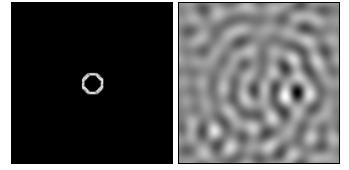
\includegraphics[width=0.6\textwidth]{img/f9.png}
    \caption{Segundo ejemplo con banda más estrecha.}
    \label{fig:pasabanda2}
\end{figure}

La simulación \ref{fig:pasabanda3} muestra el filtrado paso-banda sobre una banda de frecuencias espaciales más altas.

\begin{figure}[!htbp]
    \centering
    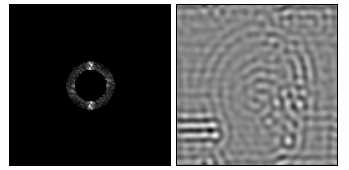
\includegraphics[width=0.6\textwidth]{img/f10.png}
    \caption{Filtrado paso-banda en una banda de frecuencias más altas.}
    \label{fig:pasabanda3}
\end{figure}

Y finalmente en \ref{fig:pasabanda4}, la misma simulación anterior pero usando de nuevo una banda de frecuencias espaciales más estrecha.

\begin{figure}[!htbp]
    \centering
    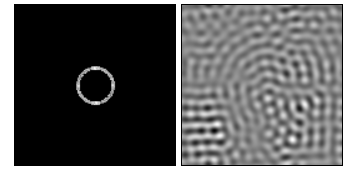
\includegraphics[width=0.6\textwidth]{img/f11.png}
    \caption{Último ejemplo con banda más estrecha.}
    \label{fig:pasabanda4}
\end{figure}

Estas simulaciones computacionales demuestran que la representación de Fourier codifica la información de la imagen de forma distribuida y global, permitiendo manipular su contenido de información espacial mediante transformaciones en el dominio transformado.




\section{Radiómica} \label{sec:radiomica}

La radiómica es un campo de la medicina de precisión que se basa en la extracción automatizada de grandes cantidades de características cuantitativas a partir de imágenes o volúmenes médicos. Estas características describen propiedades de forma, textura, intensidad y patrones espaciales, y se extraen para analizarlas posteriormente mediante técnicas estadísticas y de aprendizaje automático para encontrar correlaciones con datos clínicos, genómicos o resultados terapéuticos. El objetivo de la radiómica es convertir las imágenes en datos cuantificables y explotables que puedan ayudar en el diagnóstico, la estratificación de pacientes, la predicción de respuesta a tratamientos y la toma de decisiones clínicas personalizadas.

Este concepto se apoya en dos ideas fundamentales. En primer lugar, se asume que las características clínicas, tisulares, celulares o genómicas de un tumor se reflejan de forma fenotípica en las imágenes médicas, es decir, características internas biológicas que tienen un impacto visible y medible en la imagen. Esto implica considerar que las propiedades extraídas de la imagen están fuertemente correlacionadas con las características biológicas y clínicas del tumor. En segundo lugar, se plantea que la información proveniente de las imágenes es complementaria a la que aportan otras fuentes, como datos clínicos o genómicos, enriqueciendo así el conjunto de características tumorales estudiadas, tal como ilustra la Figura \ref{fig:radiomica-cancer}.

Tradicionalmente, la interpretación médica de las imágenes se ha basado en un análisis visual del contraste. Aunque este enfoque ha demostrado ser eficaz en el tratamiento de pacientes oncológicos, presenta limitaciones al ser cualitativo y subjetivo. La radiómica busca superar estas limitaciones mediante la cuantificación objetiva y reproducible de características, permitiendo analizar un número cada vez mayor de parámetros y modelar índices complejos de forma sistemática.

\begin{figure}[!htbp]
    \centering
    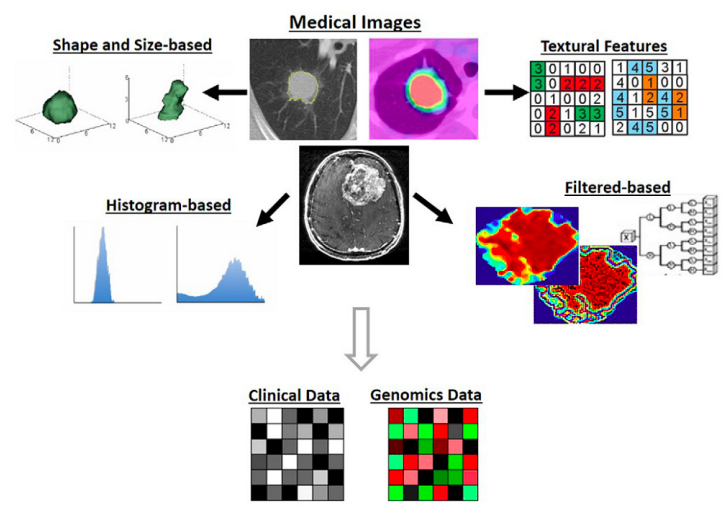
\includegraphics[width=1\textwidth]{img/radiomica_cancer.png}
    \caption{Principio de radiómica y extracción de características a partir de imágenes tumorales \parencite{demathematical} }
    \label{fig:radiomica-cancer}
\end{figure}



\subsection{Biomarcadores de imagen}
Vamos a explicar los fundamentos de la radiómica necesarios para la parte práctica de la sección \ref{chap:aa-radiomica}. En concreto vamos a explicar los biomarcadores de imagen utilizados en la parte experimental.

Esta explicación se basa en \textit{Image biomarker standardisation initiative (IBSI)}\footnote{\url{https://theibsi.github.io/}} y la documentación de \textit{PyRadiomics}\footnote{\url{https://pyradiomics.readthedocs.io/en/latest/}}. 

\subsubsection{ROI y VOI}
En radiómica se trabaja con regiones de interés (ROI, \textit{Region of Interest}) y volúmenes de interés (VOI, \textit{Volume of Interest}). La ROI es una selección bidimensional dentro de una imagen médica (como un contorno en una sola imagen o slice), mientras que la VOI es su extensión tridimensional: el conjunto de todas las ROIs a lo largo de las diferentes imágenes o cortes que forman el volumen completo. Estas regiones o volúmenes delimitan el área anatómica o la lesión sobre la que se van a calcular las características.

\subsubsection{Características de forma}
Las características de forma se basan en la ROI o VOI. Cuando se menciona la superficie del volumen, la iniciativa IBSI establece que el volumen debe representarse mediante una malla, para no sobrestimar el área de la superficie.

\paragraph{Volumen}

Existen dos tipos de volumen:

\begin{itemize}
    \item \textbf{Volumen de malla}:
    \[
    V_i = \frac{O_{ai} \cdot (O_{bi} \times O_{ci})}{6}
    \]
    
    \item \textbf{Volumen de vóxeles}:
    \[
    V = \sum_{i=1}^{N_f} V_i \tag{2.11}
    \]
\end{itemize}

\paragraph{Esfericidad de la lesión}

Mide el carácter circular definido según la ecuación:

\[
\text{sphericity} = \frac{1}{36\pi} \frac{S_{VOI}^3}{V_{VOI}^2} \tag{2.12}
\]

Donde $S_{VOI}$ y $V_{VOI}$ son respectivamente la superficie y el volumen del VOI estudiado. El factor $\frac{1}{36\pi}$ asegura que la esfericidad sea igual a 1 para una esfera.

\subsubsection{Características de primer orden}
Es posible resumir la intensidad de una imagen en un histograma. Este histograma es una función $h$ que para cada nivel de gris $i$ da el número de vóxeles que tienen esa intensidad en un VOI de tamaño $\omega = X \times Y \times Z$:

\[
h(i) = \sum_{x=1}^{X} \sum_{y=1}^{Y} \sum_{z=1}^{Z} \delta(I(x, y, z), i) \quad \text{con } i = 0,1,\ldots,G-1 \tag{2.13}
\]

donde la imagen $I$ se puede considerar como una función de tres variables $x, y, z$ con $x \in [1,X]$, $y \in [1,Y]$ y $z \in [1,Z]$. $I(x,y,z)$ puede tomar valores discretos tales como $i = 0,1,\ldots,G-1$, donde $G$ es el número total de niveles de gris. La función $\delta(j,i)$ es la función de Kronecker, definida como:

\[
\delta(j,i) =
\begin{cases}
1 & \text{si } j = i \\[6pt]
0 & \text{en otro caso}
\end{cases}
\tag{2.14}
\]

La densidad de probabilidad de intensidades $p(i)$ se obtiene así:

\[
p(i) = \frac{1}{\omega} \times h(i) \quad \text{con } i = 0,1,\ldots,G-1 \tag{2.15}
\]

El histograma de frecuencias es un resumen simple y conciso de la información estadística de primer orden contenida en la imagen. La forma del histograma es indicativa de la homogeneidad de intensidades en el VOI. El histograma de una imagen de bajo contraste se distribuye en un rango estrecho de intensidades, mientras que una imagen heterogénea corresponde a un rango amplio de intensidades.

A partir del histograma se pueden calcular varias características. Estas se definen en la tabla \ref{tab:primer_orden}. Son sencillas de calcular una vez que se ha definido la ROI o VOI.

\begin{table}[!htbp]
\centering
\renewcommand{\arraystretch}{3.0} % Más espacio entre filas
\setlength{\tabcolsep}{12pt} % Más espacio entre columnas
\caption{Principales características de primer orden.}
\label{tab:primer_orden}
\begin{tabular*}{\textwidth}{@{\extracolsep{\fill}} l l}
\toprule
\textbf{Característica} & \textbf{Fórmula} \\
\midrule
Intensidad Media & 
$\displaystyle \mu = \sum_{i=0}^{G-1} i \, p(i)$ \\

Varianza & 
$\displaystyle \sigma^2 = \sum_{i=0}^{G-1} (i - \mu)^2 \, p(i)$ \\

Asimetría & 
$\displaystyle \mu_3 = \frac{1}{\sigma^3} \sum_{i=0}^{G-1} (i - \mu)^3 \, p(i)$ \\

Curtosis & 
$\displaystyle \mu_4 = \frac{1}{\sigma^4} \sum_{i=0}^{G-1} (i - \mu)^4 \, p(i)$ \\

Energía & 
$\displaystyle E = \sum_{i=0}^{G-1} [p(i)]^2$ \\

Entropía & 
$\displaystyle H = -\sum_{i=0}^{G-1} p(i) \log_2[p(i)]$ \\

Coeficiente de Variación (COV) & 
$\displaystyle \mathrm{COV} = \frac{\sigma}{\mu}$ \\
\bottomrule
\end{tabular*}
\end{table}




\subsubsection{Características de orden superior}

La textura de una imagen corresponde a la representación matemática de la apariencia visual de una superficie, lo que permite expresar la frecuencia de repetición de un patrón o la homogeneidad de las intensidades.

En la literatura se proponen cuatro matrices principales de textura:

\begin{itemize}
    \item \textbf{Matrices de co-ocurrencia de niveles de gris (GLCM)}: introducidas por \cite{haralick2007textural}, contienen el conjunto de estadísticas de segundo orden de la imagen, caracterizando las relaciones de intensidad entre pares de vóxeles vecinos. Cuenta cuántas veces aparecen pares de valores de gris con una relación espacial específica (dirección y distancia) en la imagen. Captura la frecuencia de transiciones entre intensidades y se usa para describir textura.
    
    \item \textbf{Matriz de diferencia de niveles de gris (GLDM)}: propuesta por \cite{amadasun1989textural}, describe la diferencia de intensidad entre vecinos y contiene estadísticas de orden superior respecto a la matriz anterior. Para cada nivel de gris, cuenta cuántos grupos de píxeles adyacentes (dependientes) existen que difieren menos que un umbral dado respecto al valor central. Mide la dependencia de un píxel respecto a sus vecinos.
    
    \item \textbf{Matrices de longitud de recorrido de niveles de gris (GLRLM)}: introducidas por \cite{galloway1974texture}, caracterizan la longitud de recorrido de la misma intensidad en una dirección dada. Registra cuántos segmentos contiguos de píxeles con el mismo valor de gris hay en una dirección dada, y su longitud. Captura la uniformidad y el tamaño de estructuras en la imagen.
    
    \item \textbf{Matriz de zonas de tamaño de niveles de gris (GLSZM)}: propuesta por \cite{thibault2013advanced}, proporciona la longitud de las zonas de la misma intensidad en todas las direcciones simultáneamente. Cuenta el número de zonas conectadas (regiones de cualquier forma) de tamaño uniforme para cada nivel de gris. A diferencia del GLRLM, no depende de la dirección, y describe la distribución del tamaño de las zonas homogéneas.
\end{itemize}

Sobre las matrices anteriores se extraen diferentes características relevantes. Las Tablas \ref{tab:GLCM}, \ref{tab:GLRLMR}, \ref{tab:GLSZMZ} y \ref{tab:GLDMN} resumen las características más relevantes sobre GLCM, GLDM, GLRLM y GLSZM, respectivamente.



\begin{table}[!htbp]
\centering
\renewcommand{\arraystretch}{3.0}
\setlength{\tabcolsep}{12pt}
\caption{Características extraídas de la matriz de co-ocurrencia de niveles de gris (GLCM). $(\mu_i, \sigma_i)$ y $(\mu_j, \sigma_j)$ son la media y la varianza de las filas o columnas de la matriz $C$ de GLCM.}
\label{tab:GLCM}
\begin{tabular*}{\textwidth}{@{\extracolsep{\fill}} l l}
\toprule
\textbf{Característica} & \textbf{Fórmula} \\
\midrule
Varianza & 
$\displaystyle \sum_{i,j} C(i,j) \big[(i - \mu_x)^2 + (j - \mu_y)^2\big]$ \\

Energía & 
$\displaystyle \sum_{i,j} C(i,j)^2$ \\

Entropía & 
$\displaystyle -\sum_{i,j} C(i,j) \log C(i,j)$ \\

Correlación & 
$\displaystyle \sum_{i,j} C(i,j) \frac{(i - \mu_x)(j - \mu_y)}{\sigma_x \sigma_y}$ \\

Diferencia Absoluta & 
$\displaystyle \sum_{i,j} C(i,j) |i - j|$ \\

Contraste & 
$\displaystyle \sum_{i,j} C(i,j) (i - j)^2$ \\

Homogeneidad & 
$\displaystyle \sum_{i,j} \frac{C(i,j)}{1 + |i - j|}$ \\

IDM & 
$\displaystyle \sum_{i,j} \frac{C(i,j)}{1 + (i - j)^2}$ \\

Sombra de Conglomerado & 
$\displaystyle \sum_{i,j} C(i,j) (i + j - \mu_x - \mu_y)^3$ \\

Tendencia de Conglomerado & 
$\displaystyle \sum_{i,j} C(i,j) (i + j - \mu_x - \mu_y)^4$ \\
\bottomrule
\end{tabular*}
\end{table}


\begin{table}[!htbp]
\centering
\renewcommand{\arraystretch}{3.0}
\setlength{\tabcolsep}{12pt}
\caption{Características locales extraídas de la matriz de longitudes de recorrido de niveles de gris (GLRLM). $N_r$ es el número total de pasadas homogéneas, $G$ es el número total de niveles de gris, $N$ es el tamaño máximo de recorridos homogéneos y $R$ es la matriz de GLRLM.}
\label{tab:GLRLMR}
\begin{tabular*}{\textwidth}{@{\extracolsep{\fill}} l l}
\toprule
\textbf{Característica} & \textbf{Fórmula} \\
\midrule
SRE (Énfasis en recorridos cortas) & 
$\displaystyle \frac{1}{N_r} \sum_{i=1}^{G} \sum_{j=1}^{N} \frac{R(i,j)}{j^2}$ \\

LRE (Énfasis en recorridos largas) & 
$\displaystyle \frac{1}{N_r} \sum_{i=1}^{G} \sum_{j=1}^{N} R(i,j) \, j^2$ \\

LGRE (Énfasis en intensidades bajas) & 
$\displaystyle \frac{1}{N_r} \sum_{i=1}^{G} \sum_{j=1}^{N} \frac{R(i,j)}{i^2}$ \\

HGRE (Énfasis en intensidades altas) & 
$\displaystyle \frac{1}{N_r} \sum_{i=1}^{G} \sum_{j=1}^{N} R(i,j) \, i^2$ \\

SRLGE (SRE combinado con LGRE)& 
$\displaystyle \frac{1}{N_r} \sum_{i=1}^{G} \sum_{j=1}^{N} \frac{R(i,j)}{i^2 j^2}$ \\

SRHGE (SRE combinado con HGRE) & 
$\displaystyle \frac{1}{N_r} \sum_{i=1}^{G} \sum_{j=1}^{N} \frac{R(i,j) \, i^2}{j^2}$ \\

LRLGE (LRE combinado con LGRE)& 
$\displaystyle \frac{1}{N_r} \sum_{i=1}^{G} \sum_{j=1}^{N} \frac{R(i,j) \, j^2}{i^2}$ \\

LRHGE (LRE combinado con HGRE)& 
$\displaystyle \frac{1}{N_r} \sum_{i=1}^{G} \sum_{j=1}^{N} R(i,j) \, i^2 j^2$ \\

GLNUr (Falta de uniformidad del nivel de gris) & 
$\displaystyle \frac{1}{N_r} \sum_{i=1}^{G} \left[\sum_{j=1}^{N} R(i,j)\right]^2$ \\

RLNU (Falta de uniformidad de la longitud del recorrido)& 
$\displaystyle \frac{1}{N_r} \sum_{j=1}^{N} \left[\sum_{i=1}^{G} R(i,j)\right]^2$ \\

RP (Porcentaje de recorridos) & 
$\displaystyle \frac{N_r}{\sum_{i=1}^{G} \sum_{j=1}^{N} R(i,j) \, j}$ \\
\bottomrule
\end{tabular*}
\end{table}

\begin{table}[!htbp]
\centering
\renewcommand{\arraystretch}{3.0}
\setlength{\tabcolsep}{12pt}
\caption{Características extraídas de la matriz de zonas de tamaño de niveles de gris (GLSZM). $N_z$ es el número total de zonas homogéneas, $G$ es el número total de niveles de gris, $N$ es el tamaño máximo de zonas homogéneas y $Z$ es la matriz de GLSZM.}
\label{tab:GLSZMZ}
\begin{tabular*}{\textwidth}{@{\extracolsep{\fill}} l l}
\toprule
\textbf{Característica} & \textbf{Fórmula} \\
\midrule
SZE (Énfasis en zonas pequeñas) & 
$\displaystyle \frac{1}{N_z} \sum_{i=1}^{G} \sum_{j=1}^{N} \frac{Z(i,j)}{j^2}$ \\

LZE (Énfasis en zonas grandes) & 
$\displaystyle \frac{1}{N_z} \sum_{i=1}^{G} \sum_{j=1}^{N} Z(i,j) \, j^2$ \\

LGZE (Énfasis en intensidades bajas) & 
$\displaystyle \frac{1}{N_z} \sum_{i=1}^{G} \sum_{j=1}^{N} \frac{Z(i,j)}{i^2}$ \\

HGZE (Énfasis en intensidades altas) & 
$\displaystyle \frac{1}{N_z} \sum_{i=1}^{G} \sum_{j=1}^{N} Z(i,j) \, i^2$ \\

SZLGE (SZE combinado con LGZE) & 
$\displaystyle \frac{1}{N_z} \sum_{i=1}^{G} \sum_{j=1}^{N} \frac{Z(i,j)}{i^2 j^2}$ \\

SZHGE (SZE combinado con HGZE) & 
$\displaystyle \frac{1}{N_z} \sum_{i=1}^{G} \sum_{j=1}^{N} \frac{Z(i,j) \, i^2}{j^2}$ \\

LZLGE (LZE combinado con LGZE) & 
$\displaystyle \frac{1}{N_z} \sum_{i=1}^{G} \sum_{j=1}^{N} \frac{Z(i,j) \, j^2}{i^2}$ \\

LZHGE (LZE combinado con HGZE) & 
$\displaystyle \frac{1}{N_z} \sum_{i=1}^{G} \sum_{j=1}^{N} Z(i,j) \, i^2 j^2$ \\

GLNUz  para la no uniformidad del nivel de gris & 
$\displaystyle \frac{1}{N_z} \sum_{i=1}^{G} \left[\sum_{j=1}^{N} Z(i,j)\right]^2$ \\

ZLNU para la no uniformidad de la longitud de zona & 
$\displaystyle \frac{1}{N_z} \sum_{j=1}^{N} \left[\sum_{i=1}^{G} Z(i,j)\right]^2$ \\

ZP para el porcentaje de zonas & 
$\displaystyle \frac{N_z}{\sum_{i=1}^{G} \sum_{j=1}^{N} Z(i,j) \, j}$ \\
\bottomrule
\end{tabular*}
\end{table}


\begin{table}[!htbp]
\centering
\renewcommand{\arraystretch}{3.0}
\setlength{\tabcolsep}{12pt}
\caption{Características extraídas de la matriz de diferencia de niveles de gris (GLDM). $E$ es el número total de vóxeles en el VOI, $G$ es el número total de niveles de gris y $N$ es la matriz de GLDM.}
\label{tab:GLDMN}
\begin{tabular*}{\textwidth}{@{\extracolsep{\fill}} l l}
\toprule
\textbf{Característica} & \textbf{Fórmula} \\
\midrule
Aspereza (Coarseness) & 
$\displaystyle \frac{1}{\sum_{i=1}^{G} (N(i,1) N(i,2))}$ \\

Contraste & 
$\displaystyle \frac{1}{E  \, G(G - 1)} \left[\sum_{i=1}^{G} \sum_{j=1}^{G} N(i,1) \, N(j,1) \, (i - j)^2\right] \times \left[\sum_{i=1}^{G} N(i,2)\right]$ \\

Actividad (Busyness) & 
$\displaystyle \frac{\sum_{i=1}^{G} N(i,1) \, N(i,2)}{\sum_{i=1}^{G} \sum_{j=1}^{G} |i \, N(i,1) - j \, N(j,1)|}$ \\

Complejidad & 
$\displaystyle \sum_{i=1}^{G} \sum_{j=1}^{G} \frac{|i - j|}{E (N(i,1) + N(j,1))} \left[N(i,1) \, N(i,2) + N(j,1) \, N(j,2)\right]$ \\

Fuerza (Strength) & 
$\displaystyle \sum_{i=1}^{G} \sum_{j=1}^{G} (N(i,1) + N(j,1)) (i - j)^2 \bigg/ \sum_{i=1}^{G} N(i,2)$ \\
\bottomrule
\end{tabular*}
\end{table}

\section{La transformada de Radón: fundamento matemático de la reconstrucción tomográfica}
Aunque en este trabajo no se ha utilizado directamente la transformada de Radón, resulta relevante estudiarla por su papel fundamental en el campo de la TC. La transformada de Radón proporciona la formulación matemática que describe cómo se forman los sinogramas (la salida de un escáner CT, donde los valores de intensidad de rayos X recibidos se mapean en un gráfico con el ángulo de rotación en un eje y el desplazamiento en el sensor en el otro) a partir de las proyecciones de rayos X y, a la inversa, cómo reconstruir un corte interno del cuerpo a partir de esos datos. Comprender esta transformada permite entender en profundidad las limitaciones físicas y matemáticas de la reconstrucción tomográfica.

Mientras que es sencillo hacer una proyección 2D de un cuerpo con una radiografía simple, reconstruir un corte a partir de un sinograma, es una tarea complicada. En la Figura~\ref{fig:tecnicas-reconstrucion} se ilustran las distintas técnicas de reconstrucción utilizadas en TC.

\begin{figure}[!htbp]
    \centering
    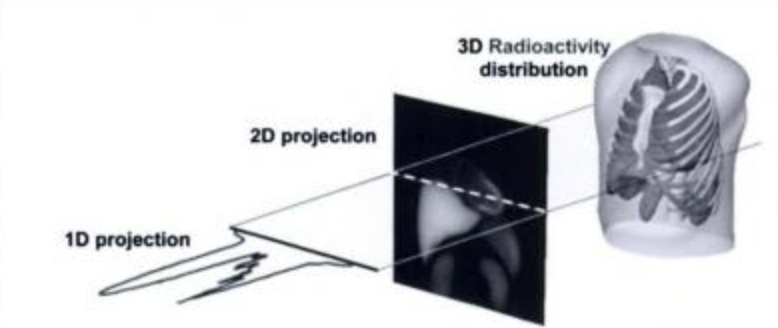
\includegraphics[width=0.8\textwidth]{img/tecnicas_reconstrucion.png}
    \caption{Técnicas de reconstrucción \parencite{bmeReconstruction}}
    \label{fig:tecnicas-reconstrucion}
\end{figure}

La transformada de radón mapea una función 2D (se han hecho extensiones 3D y ahora se usan para TC \parencite{vassholz2016new}) a otro espacio, cuyas coordenadas corresponden a la salida del sinograma de un escáner de TC.
La transformada de radón es la expresión matemática perfecta del problema de reconstrucción de TC. La Figura~\ref{fig:trans} muestra un ejemplo visual de la aplicación de esta transformada a una imagen sencilla.

\begin{figure}[!htbp]
    \centering
    \begin{subfigure}[b]{0.35\textwidth}
        \centering
        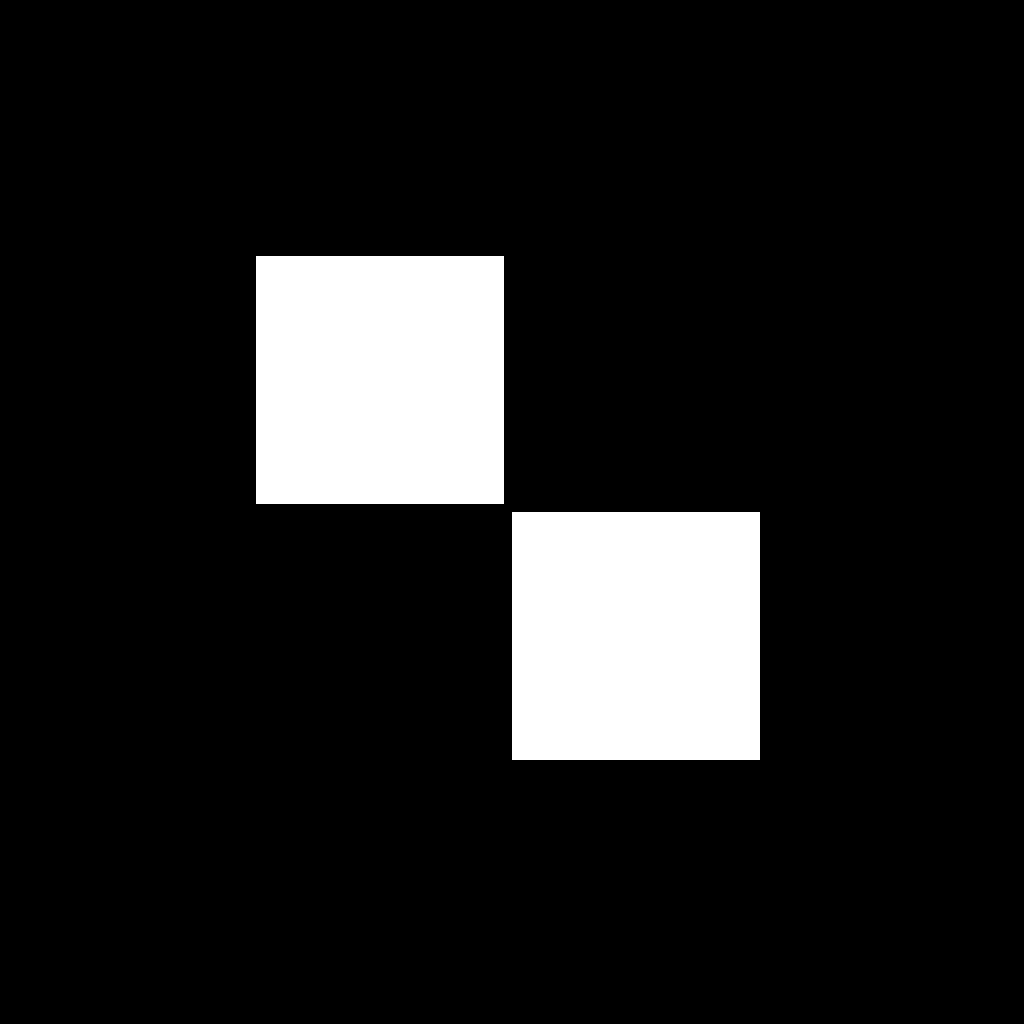
\includegraphics[width=\textwidth]{img/trans1.png}
        \caption{Imagen original cuya función binaria es igual a uno en la región blanca y a cero en la región oscura.}
        \label{fig:sinusoide_baja}
    \end{subfigure}
    \hfill
    \begin{subfigure}[b]{0.50\textwidth}
        \centering
        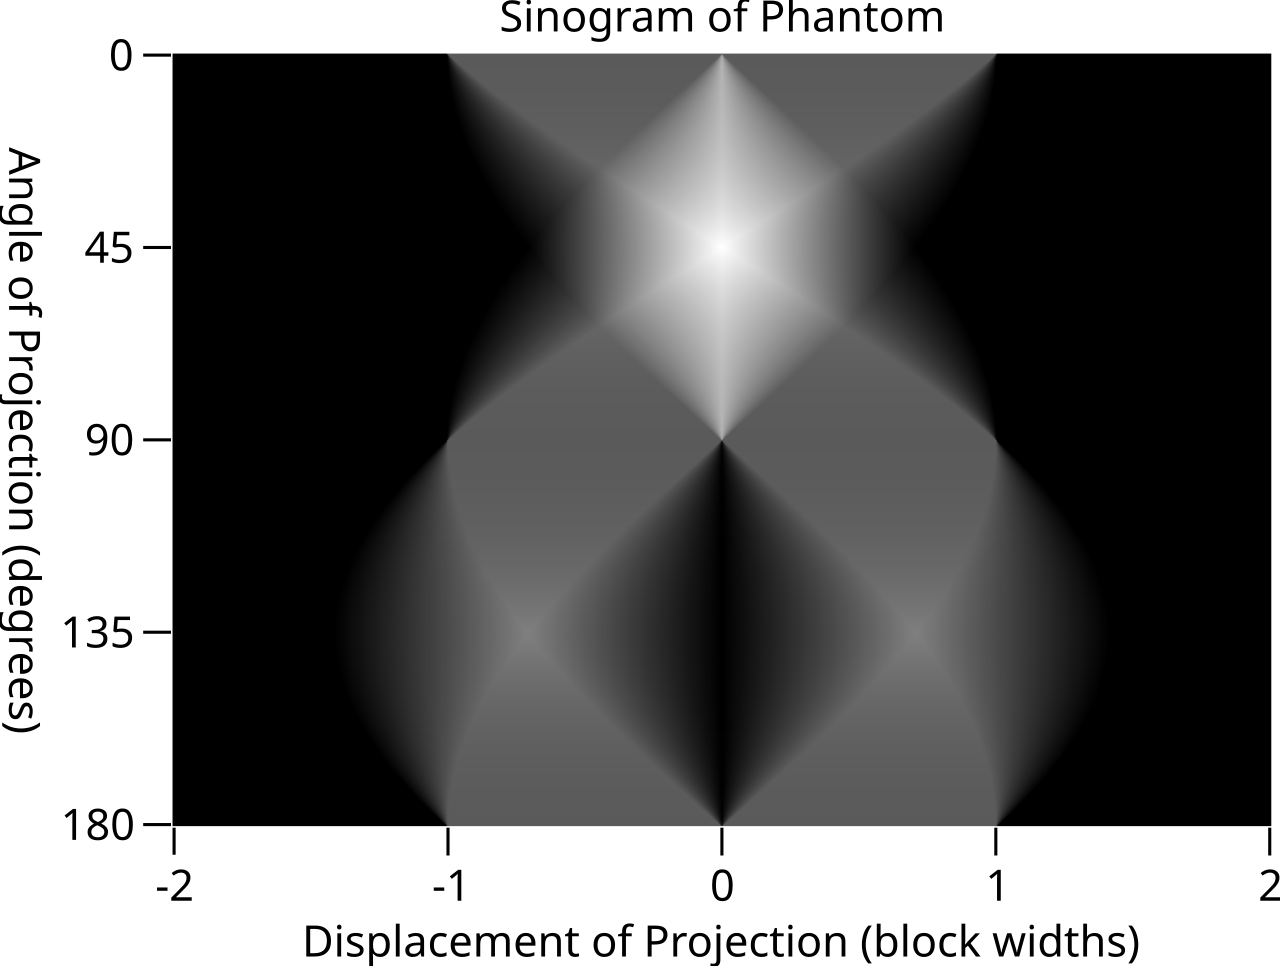
\includegraphics[width=\textwidth]{img/trans2.png}
        \caption{Transformada de Radón de la imagen anterior. Las regiones más claras indican valores mayores de la función. El negro indica cero.}
        \label{fig:sinusoide_alta}
    \end{subfigure}
    \caption{\cite{wikipediaRadon}.}
    \label{fig:trans}
\end{figure}

La transformada de radón se define como sigue para una función $g$ y su transformada de radón $\mathcal{R}_g$:

\begin{equation}
\mathcal{R}_g(x,y) = \int_{L} g(x,y) \, dl 
\end{equation}

donde $\int_{L}$ es una integral de línea (también conocida como integral de curva: integral cuya función a integrar es evaluada sobre una curva), equivalente matemático de la absorción física de un rayo X por los tejidos. $L$ está dado por:

\begin{equation}
p = x \cdot \cos \theta + y \cdot \sin \theta 
\end{equation}

con el siguiente cambio de variable: 

\[
\begin{cases}
x = p \cdot \cos \theta - q \cdot \sin \theta \\[6pt]
y = p \cdot \sin \theta + q \cdot \cos \theta
\end{cases}
\]


se puede obtener la siguiente definición integral de la transformada de Radón:

\begin{equation}
\mathcal{R}_g(p,\theta) = \int_{-\infty}^{\infty} g(p \cdot \cos \theta - q \cdot \sin \theta, \, p \cdot \sin \theta + q \cdot \cos \theta) \, dq 
\end{equation}

Un ejemplo de reconstrucción a partir del sinograma se presenta en la Figura~\ref{fig:transformada-radon}.

\begin{figure}[!htbp]
    \centering
    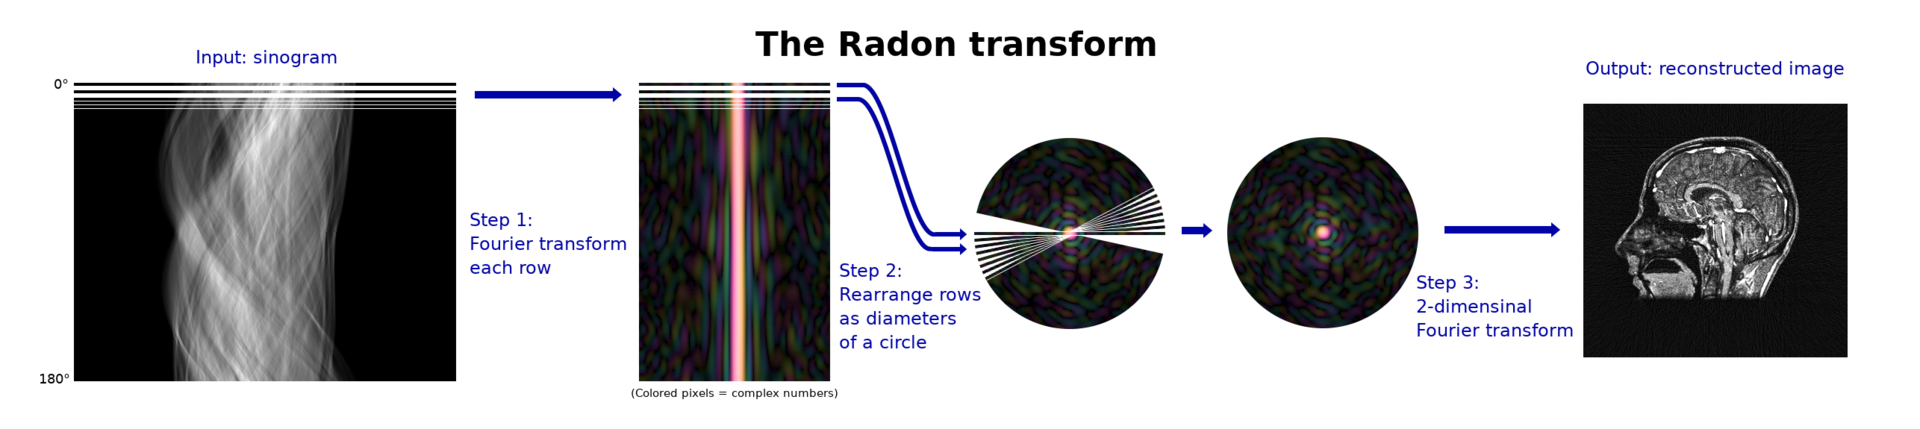
\includegraphics[width=1\textwidth]{img/transformada_radon.png}
    \caption{Reconstrucción del corte original mediante su sinograma de transformada de radón y la transformada de Fourier \parencite{wikipediaRadon}.}
    \label{fig:transformada-radon}
\end{figure}

La transformada de Radón tiene propiedades útiles análogas a las de la transformada de Fourier, por ejemplo para una función $g$ y su transformada de Radón $\mathcal{R}_g$:

\begin{itemize}
    \item Para una traslación por $(x_0, y_0)$:
\end{itemize}

\begin{equation}
g(x - x_0, y - y_0) \longleftrightarrow \mathcal{R}_g(p - x_0 \cdot \cos \theta - y_0 \cdot \sin \theta, \theta) 
\end{equation}

\begin{itemize}
    \item para una rotación por $\phi$:
    \[
    g(x \cdot \cos \phi - y \cdot \sin \phi, x \cdot \sin \phi + y \cdot \cos \phi) \longleftrightarrow \mathcal{R}_g(p, \theta + \phi) \tag{2.6}
    \]
    
    \item para una escala por un factor $\alpha$:
    \[
    g(\alpha x, \alpha y) \longleftrightarrow \frac{1}{|\alpha|} \cdot \mathcal{R}_g(\alpha p, \theta) \tag{2.7}
    \]
    
    \item conservación de la energía:
    \[
    \int_{-\infty}^{\infty} \int_{-\infty}^{\infty} g(x,y) \, dx \, dy \longleftrightarrow \int_{-\infty}^{\infty} \mathcal{R}_g(p,\theta) \, dp \tag{2.8}
    \]
\end{itemize}

Estas propiedades hacen que la transformada de Radón sea útil más allá de la reconstrucción tomográfica, como por ejemplo en el uso de funciones hash.

\subsection{Reconstrucción a partir de la transformada de Radón}

Para el caso 2D, la formulación analítica usada para la reconstrucción es la siguiente:

\[
f(\mathbf{x}) = \frac{1}{(2\pi)^2} \int_{0}^{\pi} \left(\mathcal{R}_f(\cdot,\theta) * h \right)(\langle \mathbf{x}, \mathbf{n}_\theta \rangle) \, d\theta \tag{2.9}
\]


donde $h$ es un núcleo de convolución como por ejemplo aquel cuya transformada es $\hat{h}(\omega) = |\omega|$, conocido comúnmente como \textit{filtro de rampa}.

Esta fórmula es consecuencia del \textit{teorema de la proyección en rebanadas} (projection slice theorem), que vincula la transformada de Radón con la transformada de Fourier y es además el fundamento práctico de la reconstrucción en TC.

\begin{teorema}
Para cualquier $\theta \in [0, \pi]$, la transformada de Fourier de la proyección $\mathcal{R}_g(\cdot,\theta)$ satisface:

\[
\int_{-\infty}^{\infty} \mathcal{R}_f(t, \theta) e^{-i \omega t} \, dt = \hat{f}(\omega \cos \theta, \omega \sin \theta) \tag{2.10}
\]
\end{teorema}

Lo que significa el teorema de la proyección en rebanadas es que la transformada de Fourier unidimensional de la proyección de Radón para un ángulo fijo $\theta$ corresponde a la transformada de Fourier 2D de la imagen original evaluada a lo largo de la línea radial $(\omega \cos \theta, \omega \sin \theta)$.

Sin embargo, dado que el proceso de reconstrucción es \textit{mal planteado} (ill-posed) de la misma forma que, por ejemplo, el problema de deconvolución, reconstruir la imagen original de forma perfecta es casi imposible.

Realizar una reconstrucción mejor aprovechando la capacidad de muestreo de los escáneres disponibles, mientras se toma el menor tiempo y se utilizan la menor cantidad de rayos X posible, es un enorme desafío en el procesamiento de imágenes. Se necesitan buenos algoritmos de reconstrucción en todas las tareas de reconstrucción 3D.


\endinput
%--------------------------------------------------------------------
% FIN DEL CAPÍTULO. 
%--------------------------------------------------------------------
